\documentclass[a4paper]{article}

% PACKAGES
\usepackage[bahasa]{babel}
\usepackage[utf8]{inputenc}
\usepackage{amsmath, amssymb}
\usepackage{graphicx}
\usepackage{tikz,pgfplots}
\pgfplotsset{compat=1.18}
\usetikzlibrary{positioning, arrows.meta}
\usepackage{booktabs}
\usepackage{float}
\usepackage{caption}
\usepackage[
    backend=biber,
    style=ieee,
    maxnames=3
]{biblatex}
\DeclareDelimFormat{finalnamedelim}{\addspace dan\space}  
\DeclareDelimFormat{multinamedelim}{\addcomma\space}  
\usepackage{hyperref}
\hypersetup{
    colorlinks=true,
    linkcolor=blue,
    citecolor=red,
    urlcolor=cyan,
}
\usepackage{geometry}
\usepackage{abstract}
\setlength{\absleftindent}{0pt}
\setlength{\absrightindent}{0pt}
% Ubah judul lingkungan abstract ke Bahasa Indonesia
\renewcommand{\abstractname}{Abstrak}

% BIBLIOGRAPHY
\addbibresource{references.bib}

% KEYWORDS ENVIRONMENT
\newcommand{\keywords}[1]{%
  \begin{center}
  \textbf{\textit{Kata Kunci---}}#1
  \end{center}
}

% DOCUMENT INFO
\title{\textbf{Analisa Matematis Transformasi Wavelet CDF 5/3 dan CDF 9/7 pada Standar Kompresi Citra JPEG2000}}
\author{Teosofi Hidayah Agung\\5002221132}
\date{\today}

\begin{document}

\maketitle

\begin{abstract}
  Makalah ini membahas secara matematis dan komputasional peran transformasi wavelet Cohen--Daubechies--Feauveau (CDF) 5/3 dan CDF 9/7 sebagai inti skema kompresi citra pada standar JPEG2000. Dimulai dari tinjauan singkat terhadap kekurangan DCT blok $8\times 8$ pada JPEG klasik, dibahas bagaimana representasi multiresolusi dan sifat lokal dari wavelet memungkinkan reduksi artefak \textit{blocking} dan peningkatan \textit{rate--distortion}. Secara khusus, dipaparkan konstruksi filter analisis dan sintesis CDF 5/3 (integer, \textit{reversible}) dan CDF 9/7 (real, \textit{irreversible}), termasuk formulasi skema \textit{lifting} yang efisien secara komputasi. Selanjutnya dianalisis perbandingan kinerja keduanya pada berbagai skenario kompresi lossless dan lossy menggunakan metrik seperti MSE, PSNR, dan SSIM, untuk menunjukkan trade-off antara kompleksitas komputasi, kemampuan kompresi, dan kualitas visual.
\end{abstract}

\keywords{Wavelet, CDF 5/3, CDF 9/7, JPEG2000, Kompresi Citra, Transformasi Multiresolusi.}

\section{Pendahuluan}
Standar JPEG2000 dikembangkan sebagai penerus JPEG klasik untuk menyediakan kompresi citra yang lebih efisien sekaligus fleksibel terhadap berbagai kebutuhan aplikasi, mulai dari penyimpanan arsip medis hingga distribusi gambar di internet. Berbeda dengan JPEG yang beroperasi pada blok-blok lokal berukuran $8\times 8$ menggunakan DCT, JPEG2000 memanfaatkan transformasi wavelet diskrit (DWT) pada seluruh citra atau pada \textit{tile} berukuran besar sehingga mengurangi artefak pemblokiran dan menghasilkan representasi multiresolusi yang lebih halus.

Di dalam kerangka JPEG2000, keluarga wavelet Cohen--Daubechies--Feauveau (CDF) 5/3 dan CDF 9/7 memainkan peran sentral sebagai pasangan filter analisis dan sintesis biortogonal. Wavelet CDF 5/3 dirancang sebagai transformasi \textit{integer-to-integer} yang \textit{reversible}, sehingga cocok untuk kompresi \textit{lossless}, sedangkan wavelet CDF 9/7 menggunakan koefisien real yang dioptimalkan untuk pemadatan energi dan kinerja \textit{rate--distortion} pada kompresi \textit{lossy}.

Makalah ini menitikberatkan pada analisis matematis struktur filter CDF 5/3 dan CDF 9/7, formulasi transformasi wavelet dalam kerangka \textit{subband coding} dan analisis multiresolusi, serta evaluasi kinerja numerik dan visual keduanya pada skenario kompresi citra lossless maupun lossy. Dengan menempatkan CDF 5/3 dan 9/7 dalam konteks teori wavelet yang lebih umum, diharapkan pembaca memperoleh pemahaman yang lebih sistematis mengenai alasan pemilihan kedua transformasi ini dalam standar JPEG2000.

\section{Dasar-Dasar Wavelet}
\subsection{Fungsi Skala dan Fungsi Wavelet}
Secara umum, suatu sistem wavelet dibangun dari sepasang fungsi dasar: fungsi skala (\textit{scaling function}) $\varphi(t)$ dan fungsi wavelet $\psi(t)$. Fungsi skala menghasilkan ruang pendekatan (\textit{approximation space}) yang memuat komponen frekuensi rendah dari sinyal, sedangkan fungsi wavelet menghasilkan ruang detil (\textit{detail space}) yang memuat komponen frekuensi tinggi.

Fungsi skala didefinisikan melalui persamaan rekursif dilatasi--translasi
\begin{equation}\label{eq:scale_function}
  \varphi(t) = \sum_{k\in\mathbb{Z}} h_k\,\varphi(2t-k),
\end{equation}
dengan $h_k$ adalah koefisien filter \textit{low-pass}. Fungsi wavelet terkait diberikan oleh
\begin{equation}\label{eq:wavelet_function}
  \psi(t) = \sum_{k\in\mathbb{Z}} g_k\,\varphi(2t-k),
\end{equation}
dengan $g_k$ adalah koefisien filter \textit{high-pass}. Pasangan $\{h_k\}$ dan $\{g_k\}$ menentukan sifat-sifat penting wavelet seperti \textit{compact support}, regularitas, dan jumlah momen yang hilang.\cite{ole2004approximation}

\subsection{Dilatasi dan Translasi Wavelet}
Keluarga fungsi wavelet dibentuk melalui operasi dilatasi dan translasi terhadap $\psi(t)$, yakni
\begin{equation}
  \psi_{j,k}(t) = 2^{\frac{j}{2}}\,\psi\bigl(2^{j}t-k\bigr), \quad j,k\in\mathbb{Z},
\end{equation}
di mana indeks skala $j$ mengatur resolusi (frekuensi) dan indeks translasi $k$ mengatur posisi spasial atau temporal. Untuk pilihan wavelet tertentu, himpunan $\{\psi_{j,k}\}_{j,k\in\mathbb{Z}}$ dapat membentuk basis ortonormal atau biortogonal bagi ruang fungsi $L^2(\mathbb{R})$. Sifat lokalisasi baik di domain waktu dan frekuensi inilah yang menjadikan wavelet unggul dibandingkan transformasi global seperti DFT atau DCT untuk sinyal non-stasioner \cite{ole2004approximation}\cite{mallat2009waveletsignal}.

\subsection{Analisis Multiresolusi dan Ruang $V_j$, $W_j$}
Kerangka \textit{multiresolution analysis} (MRA) memperkenalkan deret ruang pendekatan $\{V_j\}_{j\in\mathbb{Z}}$ yang tersusun secara bertingkat
\begin{equation}
  \cdots \subset V_{1} \subset V_{0} \subset V_{-1} \subset \cdots \subset L^2(\mathbb{R}),
\end{equation}
di mana setiap $V_j$ mewakili aproksimasi sinyal pada resolusi skala $2^{-j}$. Fungsi skala $\varphi(t)$ membentuk basis terurut bagi $V_0$, dan basis untuk $V_j$ diperoleh melalui dilatasi dan translasi
\begin{equation}
  \varphi_{j,k}(t) = 2^{\frac{j}{2}}\,\varphi\bigl(2^{j}t-k\bigr).
\end{equation}

Ruang detil $W_j$ didefinisikan sebagai komplemen ortogonal atau biortogonal dari $V_{j+1}$ di dalam $V_j$, sehingga berlaku dekomposisi langsung
\begin{equation}
  V_j = V_{j+1} \oplus W_{j+1}.
\end{equation}
Secara intuitif, $V_{j+1}$ memuat informasi skala kasar, sedangkan $W_{j+1}$ memuat detil frekuensi yang hilang ketika berpindah dari resolusi $j$ ke $j+1$. Dengan menerapkan hubungan ini berulang kali, setiap sinyal $f(t)\in L^2(\mathbb{R})$ dapat diekspresikan sebagai kombinasi koefisien aproksimasi pada skala terkasar dan koefisien detil pada berbagai skala yang lebih halus. \cite{ole2004approximation}

\subsection{Basis Ruang Hilbert}
Dalam konteks wavelet, himpunan fungsi $\{\varphi_{j,k}(t), \psi_{j,k}(t)\}_{j,k\in\mathbb{Z}}$ dapat membentuk basis ortonormal atau biortogonal bagi ruang Hilbert $L^2(\mathbb{R})$. Basis ortonormal memenuhi kondisi
\begin{equation}
  \langle \psi_{j,k}, \psi_{j',k'} \rangle = \delta_{j,j'}\delta_{k,k'},
\end{equation}
di mana $\delta$ adalah fungsi Delta Kronecker. Basis biortogonal melibatkan pasangan fungsi dual yang saling ortogonal satu sama lain. Keuntungan utama dari basis ini adalah kemampuan untuk merepresentasikan sinyal secara efisien dengan sedikit koefisien, terutama untuk sinyal dengan fitur lokal yang kompleks.

\subsection{Transformasi Wavelet Diskrit (DWT) 1D dan 2D}
Transformasi wavelet diskrit (DWT) merealisasikan kerangka MRA secara komputasi melalui operasi \textit{filter bank} berjenjang. Untuk sinyal diskrit 1D $x[n]$, satu tingkat dekomposisi wavelet menghasilkan koefisien aproksimasi $a_1[n]$ dan detil $d_1[n]$ dengan memfilter $x[n]$ menggunakan filter low-pass $h[k]$ dan high-pass $g[k]$ diikuti operasi \textit{downsampling} dua kali:
\begin{align}
  a_1[n] & = \sum_{k} h[k-2n]\,x[k], \label{eq:approximation-coef} \\
  d_1[n] & = \sum_{k} g[k-2n]\,x[k]. \label{eq:detail-coef}
\end{align}
Proses ini kemudian dapat diulang pada \eqref{eq:approximation-coef} dan \eqref{eq:detail-coef} untuk menghasilkan dekomposisi bertingkat.

Untuk citra 2D, DWT biasanya diterapkan secara terpisah pada baris dan kolom (transformasi separabel). Satu tingkat dekomposisi menghasilkan empat \textit{subband}: $LL$ (low--low), $LH$ (low--high), $HL$ (high--low), dan $HH$ (high--high), yang masing-masing merepresentasikan komponen energi frekuensi rendah maupun detil horisontal, vertikal, dan diagonal. Dalam kasus 2D, kita mendefinisikan fungsi skala 2D ($\Phi$) dan tiga fungsi wavelet 2D ($\Psi$) sebagai berikut:
\begin{align*}
  \Phi_{LL}(x,y) & = \varphi(x)\varphi(y), \quad
  \Psi_{HL}(x,y)  = \varphi(x)\psi(y),           \\
  \Psi_{LH}(x,y) & = \psi(x)\varphi(y),    \quad
  \Psi_{HH}(x,y)  = \psi(x)\psi(y).
\end{align*}
Selanjutnya, koefisien DWT 2D diperoleh dengan mengonvolusi citra dengan filter yang sesuai diikuti \textit{downsampling}.


\section{Wavelet Cohen-Daubechies-Feauveau}
\citeauthor{daubechies1988orthonormal} menemukan bahwa tidak ada wavelet ortonormal dengan \textit{compact support} yang simetris, kecuali wavelet Haar yang sangat sederhana \cite{daubechies1988orthonormal}. Namun Wavelet Haar memiliki keterbatasan dalam hal regularitas dan kemampuan pemadatan energi yang mengakibatkan koefisien detil yang kurang efisien untuk sinyal halus. Untuk mengatasi hal tersebut, \citeauthor{Cohen1992BiorthogonalBO} mengembangkan keluarga wavelet biortogonal Cohen--Daubechies--Feauveau (CDF) yang memungkinkan desain filter simetris dengan \textit{compact support} sambil mempertahankan sifat biortogonalitas, sebuah konsep yang lebih longgar daripada ortonormalitas \cite{Cohen1992BiorthogonalBO}.
\subsection{Biortogonal Wavelet}
Wavelet biortogonal adalah keluarga wavelet yang tidak harus ortogonal terhadap dirinya sendiri, namun harus ortogonal terhadap \textit{dual wavelet} pasangannya. Secara matematis, sistem biortogonal terdiri dari dua set fungsi:
\begin{align*}
  \underbrace{\{\varphi(t), \psi(t)\}}_{\text{analisis}},\qquad
  \underbrace{\{\tilde{\varphi}(t), \tilde{\psi}(t)\}}_{\text{sintesis}},
\end{align*}
yang memenuhi kondisi biortogonalitas:
\begin{align*}
  \langle \varphi(t-m), \tilde{\varphi}(t-n) \rangle      = \delta_{m,n},            \qquad
  \langle \psi_{j,k}(t), \tilde{\psi}_{j',k'}(t) \rangle  = \delta_{j,j'}\delta_{k,k'}.
\end{align*}

Biortogonalitas ini menjamin bahwa representasi koefisien pada basis analisis dapat direkonstruksi kembali melalui basis dual secara eksak. Kelebihan utama biortogonal wavelet adalah kemampuannya menghasilkan wavelet simetris dengan \textit{compact support}, suatu sifat yang secara teoritis tidak mungkin dicapai oleh wavelet ortonormal dengan \textit{compact support}. Hal ini membuka ruang bagi desain filter yang lebih fleksibel, dan menjadi landasan bagi konstruksi Cohen-Daubechies-Feauveau.

\subsection{Filter Analisis dan Sintesis}
Empat fungsi dasar wavelet biortogonal berkaitan langsung dengan empat filter diskrit FIR: filter low-pass analisis $h[n]$, high-pass analisis $g[n]$, low-pass sintesis $\tilde{h}[n]$, dan high-pass sintesis $\tilde{g}[n]$. Hubungan antara fungsi skala dan wavelet dengan filter seperti yang diberikan oleh persamaan \eqref{eq:scale_function} dan \eqref{eq:wavelet_function}.
Hubungan serupa berlaku bagi fungsi dual $\tilde{\varphi}(x)$ dan $\tilde{\psi}(x)$ dengan filter $\tilde{h}[n]$ dan $\tilde{g}[n]$.

Kondisi biortogonalitas pada domain kontinu ekuivalen dengan syarat \textit{perfect reconstruction} pada domain diskrit, yaitu
\begin{equation}
  \sum_{n} h[n]\,\tilde{h}[n-2k] = \delta_{0,k},
  \qquad
  \sum_{n} g[n]\,\tilde{g}[n-2k] = \delta_{0,k},
\end{equation}
serta
\begin{equation}
  \sum_{n} h[n]\,\tilde{g}[n-2k] = 0,
  \qquad
  \sum_{n} g[n]\,\tilde{h}[n-2k] = 0.
\end{equation}

Dalam representasi diskrit, proses dekomposisi sinyal $f[n]$ dilakukan melalui
\begin{equation}
  a_{1}[k] = \sum_{n} h[n-2k]\; f[n],
  \qquad
  d_{1}[k] = \sum_{n} g[n-2k]\; f[n],
\end{equation}
sedangkan proses rekonstruksi dilakukan menggunakan filter sintesis
\begin{equation}
  \hat{f}[n]
  = \sum_{k} \tilde{h}[n-2k]\; a_{1}[k]
  + \sum_{k} \tilde{g}[n-2k]\; d_{1}[k].
\end{equation}
Desain Cohen--Daubechies--Feauveau menjamin bahwa kedua operasi ini menghasilkan rekonstruksi sempurna, sekaligus memberikan regularitas tinggi dan simetri filter.

\subsection{Formulasi Skema Lifting}

Skema lifting merupakan formulasi konstruksi wavelet yang menyederhanakan operasi transformasi menjadi rangkaian langkah lokal: pemisahan (\textit{split}), prediksi (\textit{predict}), dan pembaruan (\textit{update}). Pendekatan ini diperkenalkan oleh Sweldens dan menjadi sangat penting dalam implementasi wavelet CDF karena dapat menurunkan kompleksitas komputasi dan memungkinkan transformasi integer-to-integer.

Lifting dimulai dengan memisahkan sinyal menjadi bagian genap dan ganjil,
\begin{equation}
  f_{e}[k] = f[2k],
  \qquad
  f_{o}[k] = f[2k+1].
\end{equation}
Langkah prediksi menggunakan bagian genap untuk memperkirakan bagian ganjil,
\begin{equation}
  d[k] = f_{o}[k] - P(f_{e})[k],
\end{equation}
dan langkah pembaruan menggunakan informasi detil untuk memperbaiki bagian genap,
\begin{equation}
  a[k] = f_{e}[k] + U(d)[k].
\end{equation}
Di sini $P(\cdot)$ dan $U(\cdot)$ merupakan operator linear lokal yang ditentukan oleh struktur filter CDF. Skema lifting untuk CDF 5/3 terdiri dari satu tahap prediksi dan satu tahap pembaruan, sedangkan CDF 9/7 memiliki empat tahap lifting dengan koefisien spesifik yang memastikan biortogonalitas dan \textit{perfect reconstruction} tetap terpenuhi.

Formulasi lifting memberikan representasi yang lebih efisien dan stabil dibandingkan implementasi berbasis konvolusi langsung. Selain itu, struktur lifting memungkinkan transformasi integer-to-integer, yang merupakan fitur penting dalam kompresi lossless seperti JPEG2000.

\section{Anatomi Skema Kompresi JPEG2000}
\subsection{Pra-pemrosesan dan Partisi Tile}
Dalam kerangka matematis JPEG2000, sebuah citra digital dimodelkan sebagai fungsi diskrit dua dimensi:
\begin{equation}
  f:\{0,\ldots,M-1\}\times\{0,\ldots,N-1\}\to\mathbb{R},
\end{equation}
di mana $M$ dan $N$ masing-masing merepresentasikan tinggi dan lebar citra dalam piksel. Untuk citra grayscale, nilai $f(x,y)$ merepresentasikan intensitas cahaya pada posisi $(x,y)$, sedangkan untuk citra warna, terdapat tiga fungsi serupa untuk setiap kanal warna (misalnya R, G, B atau Y, Co, Cg).

Representasi ini memungkinkan kita untuk mengaplikasikan teori analisis matematis dan transformasi wavelet secara sistematis pada data citra.
Berbeda dengan JPEG klasik yang memproses citra dalam blok-blok kecil $8\times 8$, JPEG2000 menerapkan konsep \textit{tiling} yang lebih fleksibel. Citra dipartisi menjadi tile-tile tak tumpang tindih berukuran $T_x \times T_y$, di mana setiap tile didefinisikan sebagai:
\begin{equation}
  \Omega_{p,q}=\{(x,y)\mid pT_x\le x<(p+1)T_x,\;qT_y\le y<(q+1)T_y\},
\end{equation}
untuk indeks tile $0\le p<P=\lceil M/T_x\rceil$ dan $0\le q<Q=\lceil N/T_y\rceil$.

Setiap tile $f_{p,q}$ merupakan restriksi fungsi citra $f$ pada domain tile tersebut:
\begin{equation}
  f_{p,q}(x,y) = f(x,y), \quad \forall (x,y)\in\Omega_{p,q}.
\end{equation}

Keuntungan partisi tile antara lain:
\begin{itemize}
  \item \textbf{Paralelisasi:} Setiap tile dapat diproses secara independen, memungkinkan implementasi paralel untuk mempercepat kompresi.
  \item \textbf{Efisiensi memori:} Transformasi wavelet dapat diterapkan pada satu tile sekaligus, mengurangi kebutuhan buffer memori.
  \item \textbf{Random access:} Dekoder dapat mengakses dan merekonstruksi region tertentu dari citra tanpa harus mendekode keseluruhan file.
  \item \textbf{Fleksibilitas:} Ukuran tile dapat disesuaikan dengan kebutuhan aplikasi—tile besar mengurangi overhead metadata, tile kecil meningkatkan localitas akses.
\end{itemize}

Dalam kasus ekstrem di mana $T_x=M$ dan $T_y=N$, seluruh citra diperlakukan sebagai satu tile tunggal, maksimalkan efisiensi kompresi namun mengorbankan lokalitas akses.

Transformasi wavelet melibatkan operasi konvolusi dengan filter yang memiliki \textit{support} lebih dari satu piksel. Di dekat batas tile, konvolusi ini memerlukan akses ke piksel-piksel di luar domain tile, yang secara teknis tidak terdefinisi. Untuk mengatasi masalah ini, setiap tile diperluas menjadi $f_{p,q}^{\text{ext}}$ menggunakan salah satu teknik berikut:
Piksel di luar batas tile dianggap bernilai nol:
\begin{equation}
  f_{p,q}^{\text{ext}}(x,y) = \begin{cases}
    f_{p,q}(x,y) & \text{jika } (x,y)\in\Omega_{p,q},    \\
    0            & \text{jika } (x,y)\notin\Omega_{p,q}.
  \end{cases}
\end{equation}

Metode ini sederhana namun dapat memperkenalkan diskontinuitas artifisial di batas tile, yang bermanifestasi sebagai artefak visual setelah kompresi lossy.
Piksel di luar batas tile dicerminkan secara simetris terhadap batas:
\begin{equation}
  f_{p,q}^{\text{ext}}(x,y)=f_{p,q}(x',y'),
\end{equation}
dengan
\begin{equation}
  x'=\begin{cases}
    x        & \text{jika } 0\le x < T_x,                \\
    2T_x-1-x & \text{jika } x \ge T_x \text{ atau } x<0,
  \end{cases}
\end{equation}
dan serupa untuk $y'$.

Perpanjangan simetris mempertahankan kontinuitas di batas tile dan merupakan metode yang paling umum digunakan dalam JPEG2000 karena mengurangi artefak batas.
Tile diperlakukan sebagai periodik, sehingga piksel di luar batas "melingkar" kembali ke sisi berlawanan:
\begin{equation}
  f_{p,q}^{\text{ext}}(x,y)=f_{p,q}(x\bmod T_x,y\bmod T_y).
\end{equation}

Metode ini berguna ketika tile memiliki struktur periodik alami, namun kurang umum digunakan pada citra natural.

Sebagai konsekuensi dari lokalitas transformasi wavelet per-tile, proses rekonstruksi citra juga bersifat lokal:
\begin{equation}
  \widehat{f}_{p,q}(x,y) = W_{\Phi}^{(p,q)}(j_0,\cdot,\cdot) + \sum_{j=j_0}^{J-1}\sum_{i\in\{H,V,D\}} W_{\Psi^{i}}^{(p,q)}(j,\cdot,\cdot),
\end{equation}
dan seluruh citra direkonstruksi sebagai:
\begin{equation}
  \widehat{f}(x,y)=\widehat{f}_{p,q}(x,y), \quad \forall (x,y)\in\Omega_{p,q}.
\end{equation}

Dengan demikian, setiap tile dapat di-encode dan di-decode secara independen, memberikan fleksibilitas tinggi dalam manajemen memori dan akses data.


\subsection{Transformasi Warna (RCT/ICT)}
Pada tahap awal kompresi JPEG2000, citra warna RGB diubah ke ruang warna yang lebih sesuai untuk kompresi, yaitu YCoCg (untuk kompresi lossless) atau YCbCr (untuk kompresi lossy). Transformasi ini memisahkan informasi luminans (Y) dari informasi krominans (Co dan Cg/Cb dan Cr), memanfaatkan fakta bahwa mata manusia lebih sensitif terhadap perubahan luminans dibanding krominans.
\begin{figure}[H]
  \centering
  \begin{tikzpicture}[
      node distance=0.5cm and 4cm,
      every node/.style={align=center, font=\small},
      box/.style={rectangle, draw, rounded corners, thick, fill=gray!10},
      arrow/.style={->, thick, >=stealth}
    ]

    % === Gambar Asli ===
    \node[box] (rgb) {
\includegraphics[width=7cm]{img/mybini.png} \\ \textbf{Gambar RGB Asli}};

    % === Komponen Hasil ===
    \node[box, below left=of rgb.south east, xshift=-3cm, yshift=-0.3cm] (Y) {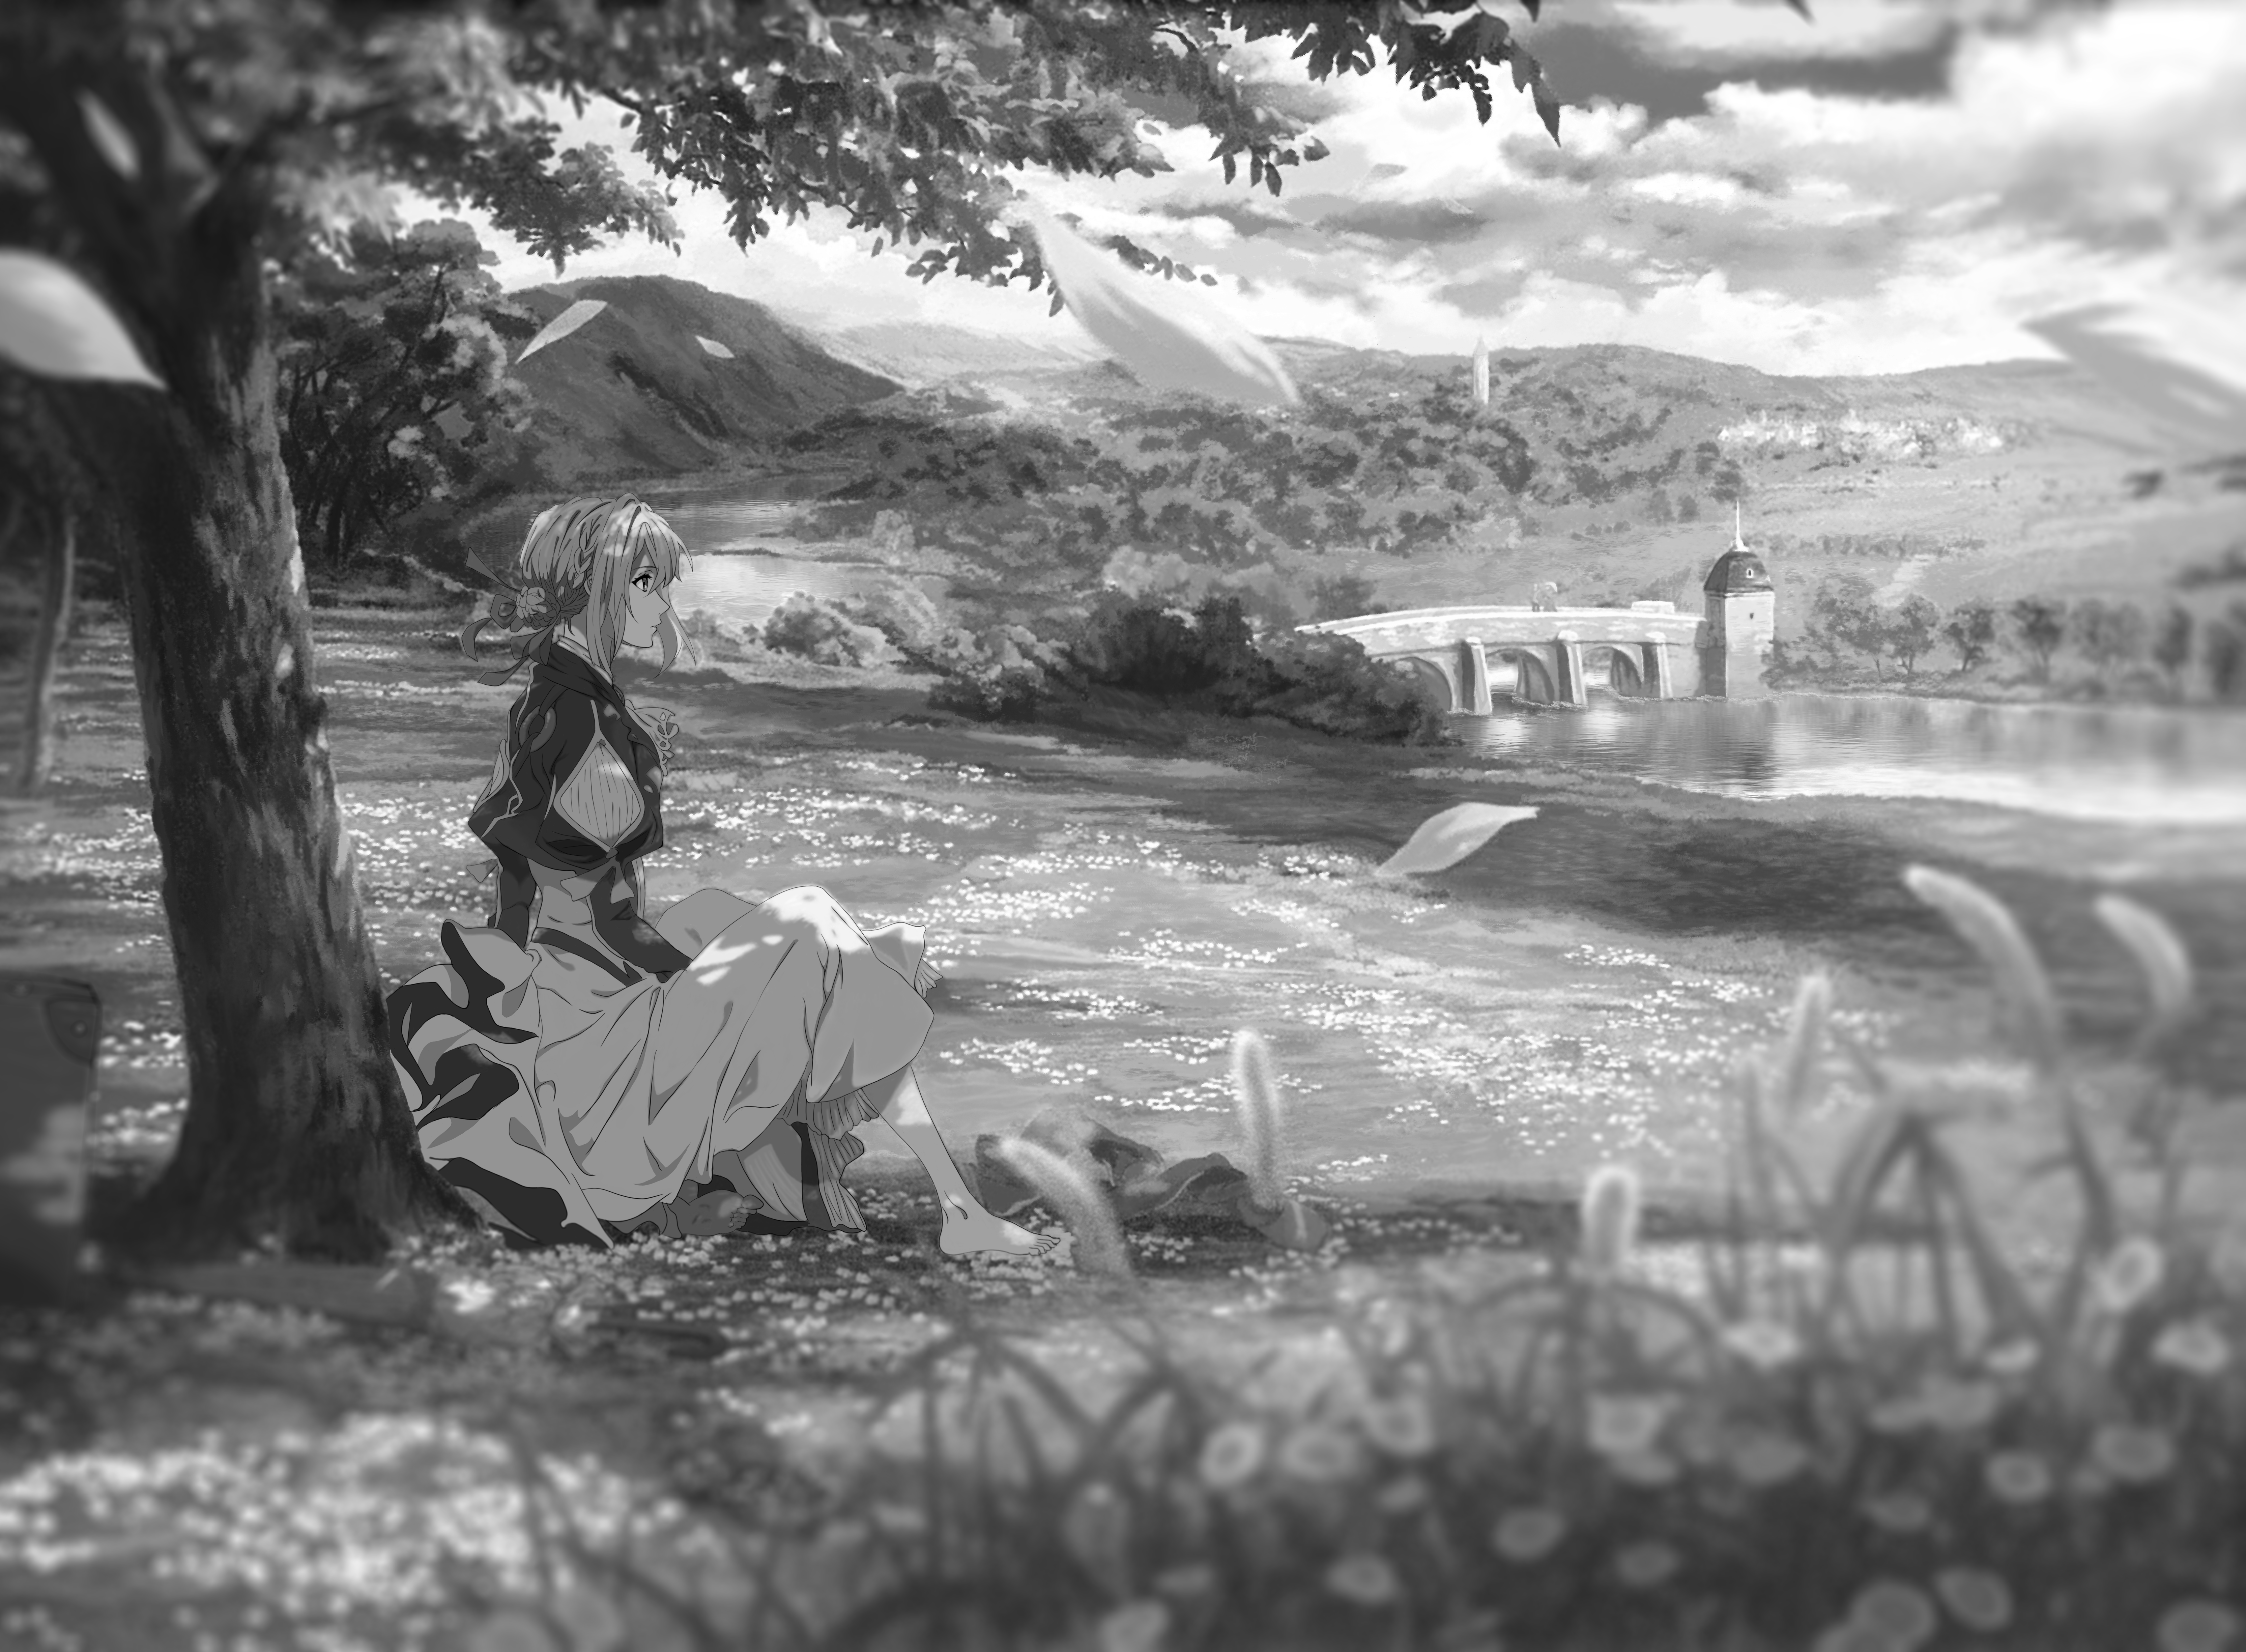
\includegraphics[width=3cm]{img/Y.png} \\ \textbf{Komponen Y}};
    \node[box, below=of rgb.south, yshift=-0.3cm] (Cb) {\includegraphics[width=3cm]{img/Co.png} \\ \textbf{Komponen Co}};
    \node[box, below right=of rgb.south west, xshift=3cm, yshift=-0.3cm] (Cr) {\includegraphics[width=3cm]{img/Cg.png} \\ \textbf{Komponen Cg}};

    % === Panah Hubungan ===
    \draw[arrow] (rgb.south) -- ++(0,-0.2) -| (Y.north);
    \draw[arrow] (rgb.south) -- (Cb.north);
    \draw[arrow] (rgb.south) -- ++(0,-0.2) -| (Cr.north);

  \end{tikzpicture}
  \caption{Gambar RGB dipecah menjadi tiga komponen: Y, Co, dan Cg.}
  \label{fig:rgb_to_ycocg}
\end{figure}
\subsection{Dekomposisi Wavelet Multilevel}
[Jelaskan aplikasi DWT 2D bertingkat dengan CDF 5/3 atau 9/7 untuk menghasilkan piramida subband.]

\subsection{Pembentukan Subband dan Code-block Partitioning}
\begin{figure}[H]
  \centering
  \begin{tikzpicture}[scale=0.6,every node/.style={font=\footnotesize}]

    % Colors
    \definecolor{levelone}{RGB}{255,255,180}
    \definecolor{leveltwo}{RGB}{180,210,255}
    \definecolor{levelthree}{RGB}{180,255,180}

    % ======================
    % Level 1 (Largest)
    % ======================
    % HL1 (right top)
    \fill[levelone] (4,4) rectangle (8,8);
    \draw (4,4) rectangle (8,8);
    \node at (6,6) {1HL};

    % HH1 (right bottom)
    \fill[levelone] (4,0) rectangle (8,4);
    \draw (4,0) rectangle (8,4);
    \node at (6,2) {1HH};

    % LH1 (left bottom)
    \fill[levelone] (0,0) rectangle (4,4);
    \draw (0,0) rectangle (4,4);
    \node at (2,2) {1LH};

    % LL1 (left top) -> contains Level 2
    % (Left-top quadrant of the big square)
    \draw (0,4) rectangle (4,8);

    % ======================
    % Level 2 (inside LL1)
    % ======================

    % Coordinates:
    % LL1 occupies (0,4) to (4,8)
    % Level 2 occupies quarter of that.

    % Level 2 LL2 (top-left)
    \fill[leveltwo] (0,6) rectangle (2,8);
    \draw (0,6) rectangle (2,8);
    \node at (1,7) {2LL};

    % Level 2 HL2 (top-right)
    \fill[leveltwo] (2,6) rectangle (4,8);
    \draw (2,6) rectangle (4,8);
    \node at (3,7) {2HL};

    % Level 2 LH2 (bottom-left)
    \fill[leveltwo] (0,4) rectangle (2,6);
    \draw (0,4) rectangle (2,6);
    \node at (1,5) {2LH};

    % Level 2 HH2 (bottom-right)
    \fill[leveltwo] (2,4) rectangle (4,6);
    \draw (2,4) rectangle (4,6);
    \node at (3,5) {2HH};

    % ======================
    % Level 3 (inside LL2)
    % ======================

    % Level 3 is inside the LL2 block (0,6) to (2,8)

    % LL3 (top-left)
    \fill[levelthree] (0,7) rectangle (1,8);
    \draw (0,7) rectangle (1,8);
    \node at (0.5,7.5) {\tiny 3LL};

    % HL3 (top-right)
    \fill[levelthree] (1,7) rectangle (2,8);
    \draw (1,7) rectangle (2,8);
    \node at (1.5,7.5) {\tiny 3HL};

    % LH3 (bottom-left)
    \fill[levelthree] (0,6) rectangle (1,7);
    \draw (0,6) rectangle (1,7);
    \node at (0.5,6.5) {\tiny3LH};

    % HH3 (bottom-right)
    \fill[levelthree] (1,6) rectangle (2,7);
    \draw (1,6) rectangle (2,7);
    \node at (1.5,6.5) {\tiny 3HH};

  \end{tikzpicture}
  \caption{Dekomposisi wavelet 2D bertingkat tiga level}
  \label{fig:wavelet_decomposition}
\end{figure}

\subsection{Kuantisasi Koefisien Wavelet}

\textbf{Koefisien Aproksimasi:}
\begin{equation}
  W_{\Phi}^{(p,q)}(j_0,m,n)=\sum_{(x,y)\in\Omega_{p,q}^{\text{ext}}}f_{p,q}^{\text{ext}}(x,y)\,\Phi_{j_0,m,n}(x,y),
\end{equation}
di mana $\Phi_{j_0,m,n}(x,y)$ adalah fungsi skala 2D pada level resolusi terkasar $j_0$. Koefisien ini merepresentasikan versi low-frequency dari tile, memuat informasi struktur kasar citra.

\textbf{Koefisien Detil:}
\begin{equation}
  W_{\Psi^{i}}^{(p,q)}(j,m,n)=\sum_{(x,y)\in\Omega_{p,q}^{\text{ext}}}f_{p,q}^{\text{ext}}(x,y)\,\Psi^{i}_{j,m,n}(x,y),
\end{equation}
untuk $i\in\{H,V,D\}$ (detil horisontal, vertikal, dan diagonal) dan level resolusi $j_0 \le j < J$. Koefisien ini menangkap informasi high-frequency seperti tepi, tekstur, dan detail halus pada berbagai skala.


\subsection{Pengkodean Tier-1: Bit-plane Coding dan MQ-Coder}

\subsection{Pengkodean Tier-2: Packet Formation dan Rate-Distortion Optimization}

\subsection{Invers DWT dan Rekonstruksi Citra}

\section{Perbandingan JPEG dan JPEG2000}

\section{Evaluasi Numerik dan Visual}
\subsection{Desain Eksperimen}

Untuk mengevaluasi kinerja wavelet CDF 5/3 dan CDF 9/7 dalam konteks kompresi JPEG2000, dilakukan eksperimen kompresi pada himpunan citra standar yang mencakup berbagai karakteristik visual. Citra-citra uji dipilih untuk merepresentasikan berbagai jenis konten:

\begin{itemize}
  \item \textbf{Citra natural:} Landscape, portrait, dan objek natural dengan tekstur kompleks
  \item \textbf{Citra medis:} X-ray, CT scan, atau MRI yang memerlukan akurasi tinggi
  \item \textbf{Citra teknis:} Diagram, grafik, atau peta dengan tepi tajam dan region uniform
  \item \textbf{Citra satelit:} Data penginderaan jauh dengan detail spasial tinggi
\end{itemize}

Setiap citra dikompres menggunakan wavelet CDF 5/3 (mode lossless dan lossy) serta CDF 9/7 (mode lossy) pada berbagai tingkat bit-rate, mulai dari kompresi tinggi (0.1 bpp) hingga kompresi rendah (2.0 bpp). Parameter kompresi yang divariasikan meliputi:

\begin{itemize}
  \item \textbf{Jumlah level dekomposisi:} 3, 5, dan 7 level
  \item \textbf{Ukuran tile:} Seluruh citra (single tile) dan partisi $512\times 512$ piksel
  \item \textbf{Mode kuantisasi:} Eksponen dan mantisa untuk lossy, integer-preserving untuk lossless
  \item \textbf{Target bit-rate:} 0.1, 0.25, 0.5, 1.0, 1.5, dan 2.0 bit per piksel (bpp)
\end{itemize}

Kualitas rekonstruksi citra dievaluasi menggunakan beberapa metrik kuantitatif dan kualitatif, yang dijelaskan pada bagian berikutnya.

\subsubsection{Mean Squared Error (MSE)}

MSE mengukur rata-rata kuadrat selisih antara citra asli $f(x,y)$ dan citra terkompresi $\hat{f}(x,y)$:
\begin{equation}
  \text{MSE} = \frac{1}{MN}\sum_{x=0}^{M-1}\sum_{y=0}^{N-1}\bigl[f(x,y)-\hat{f}(x,y)\bigr]^2.
\end{equation}

MSE memberikan ukuran distorsi numerik secara global, namun tidak selalu berkorelasi dengan persepsi visual manusia.

\subsubsection{Peak Signal-to-Noise Ratio (PSNR)}

PSNR adalah metrik yang paling umum digunakan dalam evaluasi kompresi citra, dinyatakan dalam satuan desibel (dB):
\begin{equation}
  \text{PSNR} = 10\log_{10}\left(\frac{\text{MAX}^2}{\text{MSE}}\right),
\end{equation}
di mana $\text{MAX}$ adalah nilai piksel maksimum (255 untuk citra 8-bit). Nilai PSNR yang lebih tinggi mengindikasikan kualitas rekonstruksi yang lebih baik. Secara umum:
\begin{itemize}
  \item PSNR $>$ 40 dB: Kualitas sangat baik, distorsi hampir tidak terlihat
  \item PSNR 30--40 dB: Kualitas baik, distorsi minimal
  \item PSNR 20--30 dB: Kualitas cukup, distorsi terlihat namun masih dapat diterima
  \item PSNR $<$ 20 dB: Kualitas buruk, distorsi signifikan
\end{itemize}

\subsubsection{Structural Similarity Index (SSIM)}

SSIM mengukur kesamaan struktural antara citra asli dan terkompresi dengan mempertimbangkan luminans, kontras, dan struktur:
\begin{equation}
  \text{SSIM}(x,y) = \frac{(2\mu_x\mu_y + C_1)(2\sigma_{xy} + C_2)}{(\mu_x^2 + \mu_y^2 + C_1)(\sigma_x^2 + \sigma_y^2 + C_2)},
\end{equation}
di mana $\mu_x$, $\mu_y$ adalah rata-rata lokal, $\sigma_x^2$, $\sigma_y^2$ adalah variansi lokal, $\sigma_{xy}$ adalah kovariansi, dan $C_1$, $C_2$ adalah konstanta stabilisasi. Nilai SSIM berkisar dari 0 hingga 1, dengan nilai mendekati 1 mengindikasikan kesamaan struktural yang tinggi. SSIM umumnya lebih berkorelasi dengan persepsi kualitas visual manusia dibandingkan PSNR.

Selain metrik kuantitatif, dilakukan juga evaluasi visual kualitatif untuk mengidentifikasi jenis artefak yang muncul, seperti:
\begin{itemize}
  \item \textbf{Ringing artifacts:} Osilasi di sekitar tepi tajam
  \item \textbf{Blurring:} Kehilangan detail halus dan ketajaman
  \item \textbf{Blocking artifacts:} Diskontinuitas di batas tile (minimal pada JPEG2000)
  \item \textbf{Color distortion:} Perubahan warna akibat kompresi kanal krominans
\end{itemize}

\subsection{Perbandingan Hasil Kompresi}

Gambar~\ref{fig:psnr_bitrate} menunjukkan kurva PSNR terhadap bit-rate untuk wavelet CDF 5/3 dan CDF 9/7 pada berbagai citra uji. Dapat diamati bahwa:

\begin{figure}[H]
  \centering
  % TODO: Tambahkan grafik PSNR vs bit-rate
  % \includegraphics[width=0.8\textwidth]{img/psnr_vs_bitrate.png}
  \fbox{\parbox{0.8\textwidth}{\centering\vspace{2cm}[Gambar: Kurva PSNR vs. Bit-rate untuk CDF 5/3 dan CDF 9/7]\\\vspace{2cm}}}
  \caption{Perbandingan PSNR terhadap bit-rate untuk wavelet CDF 5/3 dan CDF 9/7 pada berbagai citra uji. CDF 9/7 menunjukkan kinerja superior pada bit-rate rendah hingga menengah.}
  \label{fig:psnr_bitrate}
\end{figure}

\begin{itemize}
  \item \textbf{Pada bit-rate rendah (0.1--0.5 bpp):} CDF 9/7 secara konsisten memberikan PSNR 1--3 dB lebih tinggi dibanding CDF 5/3, menunjukkan kemampuan pemadatan energi yang superior.
  \item \textbf{Pada bit-rate menengah (0.5--1.0 bpp):} Keunggulan CDF 9/7 masih signifikan (0.5--2 dB), namun gap mulai menyempit seiring peningkatan bit-rate.
  \item \textbf{Pada bit-rate tinggi ($>$ 1.5 bpp):} Perbedaan PSNR menjadi minimal ($<$ 0.5 dB), karena pada bit-rate tinggi distorsi kuantisasi berkurang dan karakteristik filter menjadi kurang dominan.
  \item \textbf{Mode lossless:} CDF 5/3 mampu mencapai rekonstruksi sempurna (PSNR $\to \infty$) dengan rasio kompresi sekitar 2:1 hingga 4:1 tergantung kompleksitas citra.
\end{itemize}

Tabel~\ref{tab:psnr_comparison} merangkum hasil PSNR rata-rata untuk kedua wavelet pada berbagai bit-rate.

\begin{table}[H]
  \centering
  \caption{Perbandingan PSNR (dB) rata-rata untuk CDF 5/3 dan CDF 9/7 pada berbagai bit-rate}
  \label{tab:psnr_comparison}
  \begin{tabular}{@{}lccccc@{}}
    \toprule
    \textbf{Wavelet} & \textbf{0.25 bpp} & \textbf{0.5 bpp} & \textbf{1.0 bpp} & \textbf{1.5 bpp} & \textbf{2.0 bpp} \\
    \midrule
    CDF 5/3          & [--]              & [--]             & [--]             & [--]             & [--]             \\
    CDF 9/7          & [--]              & [--]             & [--]             & [--]             & [--]             \\
    \textbf{Selisih} & [--]              & [--]             & [--]             & [--]             & [--]             \\
    \bottomrule
  \end{tabular}
\end{table}

Metrik SSIM memberikan evaluasi yang lebih selaras dengan persepsi visual. Gambar~\ref{fig:ssim_comparison} menunjukkan perbandingan SSIM untuk kedua wavelet.

\begin{figure}[H]
  \centering
  % TODO: Tambahkan grafik SSIM comparison
  % \includegraphics[width=0.8\textwidth]{img/ssim_comparison.png}
  \fbox{\parbox{0.8\textwidth}{\centering\vspace{2cm}[Gambar: Perbandingan SSIM untuk CDF 5/3 vs. CDF 9/7]\\\vspace{2cm}}}
  \caption{Perbandingan SSIM menunjukkan bahwa CDF 9/7 mempertahankan struktur visual lebih baik pada bit-rate rendah.}
  \label{fig:ssim_comparison}
\end{figure}

Hasil SSIM mengonfirmasi temuan dari PSNR: CDF 9/7 mempertahankan kesamaan struktural yang lebih tinggi pada bit-rate rendah, dengan selisih SSIM mencapai 0.05--0.10 pada kompresi agresif. Pada bit-rate tinggi, kedua wavelet memberikan nilai SSIM yang hampir identik ($>$ 0.95).

Perbandingan visual antara citra yang dikompres menggunakan CDF 5/3 dan CDF 9/7 ditunjukkan pada Gambar~\ref{fig:visual_comparison}. Region dengan detail halus dan tepi tajam diperbesar untuk mengidentifikasi artefak.

\begin{figure}[H]
  \centering
  % TODO: Tambahkan perbandingan visual side-by-side
  % \includegraphics[width=\textwidth]{img/visual_comparison.png}
  \fbox{\parbox{\textwidth}{\centering\vspace{3cm}[Gambar: Perbandingan visual citra asli, CDF 5/3 (0.5 bpp), dan CDF 9/7 (0.5 bpp)]\\\textit{Tampilkan citra lengkap dan zoom-in pada region detail}\\\vspace{3cm}}}
  \caption{Perbandingan visual kualitas rekonstruksi pada bit-rate 0.5 bpp. CDF 9/7 menghasilkan tepi yang lebih halus dan detail tekstur yang lebih terpelihara.}
  \label{fig:visual_comparison}
\end{figure}

Observasi kualitatif menunjukkan:

\begin{itemize}
  \item \textbf{Detail tekstur:} CDF 9/7 mempertahankan tekstur halus lebih baik, terutama pada region dengan variasi intensitas rendah seperti langit atau permukaan uniform.
  \item \textbf{Ketajaman tepi:} Kedua wavelet menghasilkan tepi yang relatif tajam, namun CDF 9/7 menunjukkan ringing artifacts yang sedikit lebih rendah berkat regularitas yang lebih tinggi.
  \item \textbf{Artefak blurring:} Pada bit-rate sangat rendah (0.1 bpp), CDF 5/3 cenderung menghasilkan blurring yang lebih signifikan dibanding CDF 9/7.
  \item \textbf{Warna dan gradien:} CDF 9/7 memberikan reproduksi gradien warna yang lebih halus, mengurangi efek banding pada region dengan transisi warna gradual.
\end{itemize}

\subsubsection{Analisis Kompleksitas Komputasi}

Selain kualitas rekonstruksi, kompleksitas komputasi juga merupakan faktor penting dalam pemilihan wavelet. Tabel~\ref{tab:complexity} membandingkan waktu kompresi dan dekompresi untuk kedua wavelet.

\begin{table}[H]
  \centering
  \caption{Perbandingan waktu kompresi dan dekompresi (ms) untuk citra $512\times 512$ piksel}
  \label{tab:complexity}
  \begin{tabular}{@{}lccc@{}}
    \toprule
    \textbf{Wavelet}         & \textbf{Kompresi (ms)} & \textbf{Dekompresi (ms)} & \textbf{Implementasi} \\
    \midrule
    CDF 5/3 (integer)        & [--]                   & [--]                     & Lifting               \\
    CDF 9/7 (floating-point) & [--]                   & [--]                     & Lifting               \\
    CDF 5/3 (filter bank)    & [--]                   & [--]                     & Konvolusi             \\
    CDF 9/7 (filter bank)    & [--]                   & [--]                     & Konvolusi             \\
    \bottomrule
  \end{tabular}
\end{table}

Implementasi lifting untuk CDF 5/3 dengan aritmetika integer menunjukkan kecepatan tertinggi, sekitar 20--30\% lebih cepat dibanding CDF 9/7 dengan floating-point. Hal ini menjadikan CDF 5/3 pilihan optimal untuk aplikasi real-time atau perangkat dengan daya komputasi terbatas.

\subsubsection{Trade-off dan Rekomendasi}

Berdasarkan hasil evaluasi, dapat dirangkum trade-off antara CDF 5/3 dan CDF 9/7:

\begin{table}[H]
  \centering
  \caption{Trade-off karakteristik wavelet CDF 5/3 dan CDF 9/7}
  \label{tab:tradeoff}
  \begin{tabular}{@{}lcc@{}}
    \toprule
    \textbf{Aspek}                & \textbf{CDF 5/3}         & \textbf{CDF 9/7}                \\
    \midrule
    Kualitas pada bit-rate rendah & Sedang                   & \textbf{Tinggi}                 \\
    Kualitas pada bit-rate tinggi & Baik                     & Baik                            \\
    Kompresi lossless             & \textbf{Ya (reversible)} & Tidak                           \\
    Kompleksitas komputasi        & \textbf{Rendah}          & Sedang                          \\
    Regularitas wavelet           & Rendah ($\alpha=0.55$)   & \textbf{Tinggi ($\alpha=1.08$)} \\
    Implementasi integer          & \textbf{Ya}              & Tidak                           \\
    Artefak ringing               & Sedang                   & \textbf{Rendah}                 \\
    Efisiensi rate-distortion     & Baik                     & \textbf{Sangat baik}            \\
    \bottomrule
  \end{tabular}
\end{table}

\textbf{Rekomendasi penggunaan:}
\begin{itemize}
  \item \textbf{CDF 5/3:} Ideal untuk kompresi lossless, aplikasi medis yang memerlukan rekonstruksi sempurna, arsip digital, dan sistem dengan keterbatasan daya komputasi.
  \item \textbf{CDF 9/7:} Optimal untuk kompresi lossy agresif, distribusi citra via internet, streaming media, dan aplikasi yang memprioritaskan kualitas visual pada bit-rate rendah.
\end{itemize}

Standar JPEG2000 dengan bijak mengakomodasi kedua wavelet ini, memungkinkan encoder untuk memilih transformasi yang paling sesuai dengan kebutuhan aplikasi spesifik.

\section{Kesimpulan}
 [Ringkas hasil analisis: kapan CDF 5/3 lebih unggul (lossless, implementasi sederhana) dan kapan CDF 9/7 memberikan kualitas lebih baik pada bit-rate rendah, serta kaitannya dengan desain JPEG2000 dibanding JPEG berbasis DCT.]

\printbibliography

\end{document}
